\documentclass[letterpaper]{article}

\usepackage{hw}
\usepackage{bm}
\usepackage{amsmath}
\usepackage{graphicx}
\usepackage[colorlinks=true,urlcolor=blue]{hyperref}
\usepackage{geometry}
\geometry{margin=1in}
\usepackage{multicol}
\usepackage{paralist}
\usepackage{todonotes}
\setlength{\marginparwidth}{2.15cm}
\usepackage{booktabs}
\usepackage{enumitem}
\usepackage{cleveref}
\usepackage{pdfpages}
\usepackage{fancyhdr}
\usepackage{verbatim}
\usepackage{tikz}
\usetikzlibrary{arrows}

%\DeclareMathOperator*{\argmin}{arg\,min}
%\DeclareMathOperator*{\argmax}{arg\,max}

\def \issoln {1}

% Some commands to allow solutions to be embedded in the assignment file.
\ifcsname issoln\endcsname \else \def\issoln{0} \fi
\newcommand{\soln}[1]
{
  \if\issoln 1
  \textbf{Solution:}
  #1
  \fi
}

\newcommand{\email}[1]{\href{mailto:#1@cs.cmu.edu}{#1}}

\pagestyle{fancy}
\lhead{AID :: \email{jarulraj}, \email{nkshah}}

\begin{document}

\section*{}
\begin{center}
  \centerline{\textsc{\LARGE Homework Assignment 3{\if\issoln 3 Solutions \else \fi}}}
  \vspace{1em}
  \textsc{\large CMU 15-745: Optimizing Compilers (Spring 2015)} \\
  \vspace{3em}
  \centerline{\large{Joy Arulraj (\email{jarulraj}), Nisarg Shah (\email{nkshah})}}
  \vspace{1em}
\end{center}

%\section{LICM: Loop Invariant Code Motion}

\subsection{Dominance Information}

We use the following data flow equations to compute dominance information using the
data flow framework. \\

$\operatorname{Dom}(n_o) = \left \{ n_o \right \}$

$\operatorname{Dom}(n) = \left ( \bigcap_{p \in \text{preds}(n)}^{} \operatorname{Dom}(p) \right ) \bigcup^{} \left \{ n \right \}$,
where $n_o$ is the start node.

\subsection{Finding Invariant Instructions}

We use the following check to determine if an LLVM Instruction pointer I is invariant :\\

\texttt{isSafeToSpeculativelyExecute(I) \&\& !I->mayReadFromMemory() \&\& !isa<LandingPadInst>(I)}\\

This is because TODO

\subsection{LICM Implementation}

TODO

\subsection{Microbenchmarks}

\begin{table}[!ht]
\centering
\begin{tabular}{c|l|l}
  \toprule
  \textbf{Benchmark} & \textbf{Instruction Count} & \textbf{Transformed Instruction Count} \\
  \midrule
  licm-test-1 & 9887 & 9857 \\ 
  licm-test-2 & 797  & 405 \\
  licm-test-3 & 9406 & 9306 \\ 
  \bottomrule
\end{tabular}
\caption{Comparison between default bitcode's dynamic instruction count and transformed
  bitcode's dynamic instruction count.}
\end{table}  


\section{Dead Code Elimination}

\subsection{DCE Implementation}

To identify the set of faint instructions, we first identify the complementary set of \textbf{strongly live instructions}.
A strongly live instruction is a instruction that is either live by definition or is used in the assignment of another
strongly live instruction.
If a instruction is not strongly live, then it is a \textbf{faint instruction}.
That is, we can remove that instruction.

For any instruction $s$, let $x$ be variable in the LHS. Let $GEN_s$ be the set of variables in the RHS (like the live variable analysis) and
let $KILL_s = \{x\}$. We use the following transfer function, where we \textbf{alter data flow only if $x$ is strongly live}. That is :

\[
IN(s) = \left\{ 
\begin{array}{ll}
GEN_s \cup (OUT(s)-KILL_s) & \mbox{if } x \in OUT(s),\\
OUT(s) & \mbox{if } x \notin OUT(s).
\end{array}
\right.
\]

Now, during our data flow analysis, once we compute $OUT(B)$ for a basic block $B$, we iterate through the instructions of $B$ in the reverse order, and apply the transfer function given above. When we reach the first instruction of the block, its $IN$ will give us $IN(B)$. It seems that unlike the transfer function of live variable analysis, this transfer function is not composable (i.e., after composing over multiple instructions in the block, its final form is not of the same type $f(x) = GEN_x \cup (x-KILL_x)$) because the instructions on which we alter the data flow depends on $OUT(B)$ itself.\\  

We use the following check to determine if an LLVM Instruction pointer I is live.

\texttt{isa<TerminatorInst>() || isa<DbgInfoIntrinsic>(I) || \\  isa<LandingPadInst>(I) || I->mayHaveSideEffects()} or if I is used by any Instruction that is also live. 

We finally erase all the instructions that are faint.

\subsection{Microbenchmarks}

\begin{table}[!ht]
\centering
\begin{tabular}{c|l|l}
  \toprule
  \textbf{Benchmark} & \textbf{Instruction Count} & \textbf{Transformed Instruction Count} \\
  \midrule
  dce-test-1 & 7  & 6  \\ 
  dce-test-2 & 20 & 16 \\
  dce-test-3 & 4  & 2  \\
  dce-test-4 & 2  & 1  \\
  \bottomrule
\end{tabular}
\caption{Comparison between default bitcode's dynamic instruction count and transformed
  bitcode's dynamic instruction count.}
\end{table}  

\newpage

%%% Local Variables:
%%% mode: latex
%%% TeX-master: "asst1"
%%% End:

%\section{Register Allocation}

The annotated CFG and the associated interference graph are shown below. 

We first identify the live ranges of all the variables. We split
pseudo-registers into live ranges to create an interference graph that
is easier to color.

We observe that the graph has a 5-clique comprising of $\{y, x_2, s_1, t, u \}$.
Hence, there is no possible 4-coloring for the graph.

We then compute the spilling cost for all the variables involved in the clique.
We note that either $x_2$ or $u$ can be spilled with minimal cost.
After spilling, say $u$, we provide a 4-coloring of the graph in the figure.
Thus, it is possible to allocate the variables in this case to 4 physical
registers after spilling $u$.

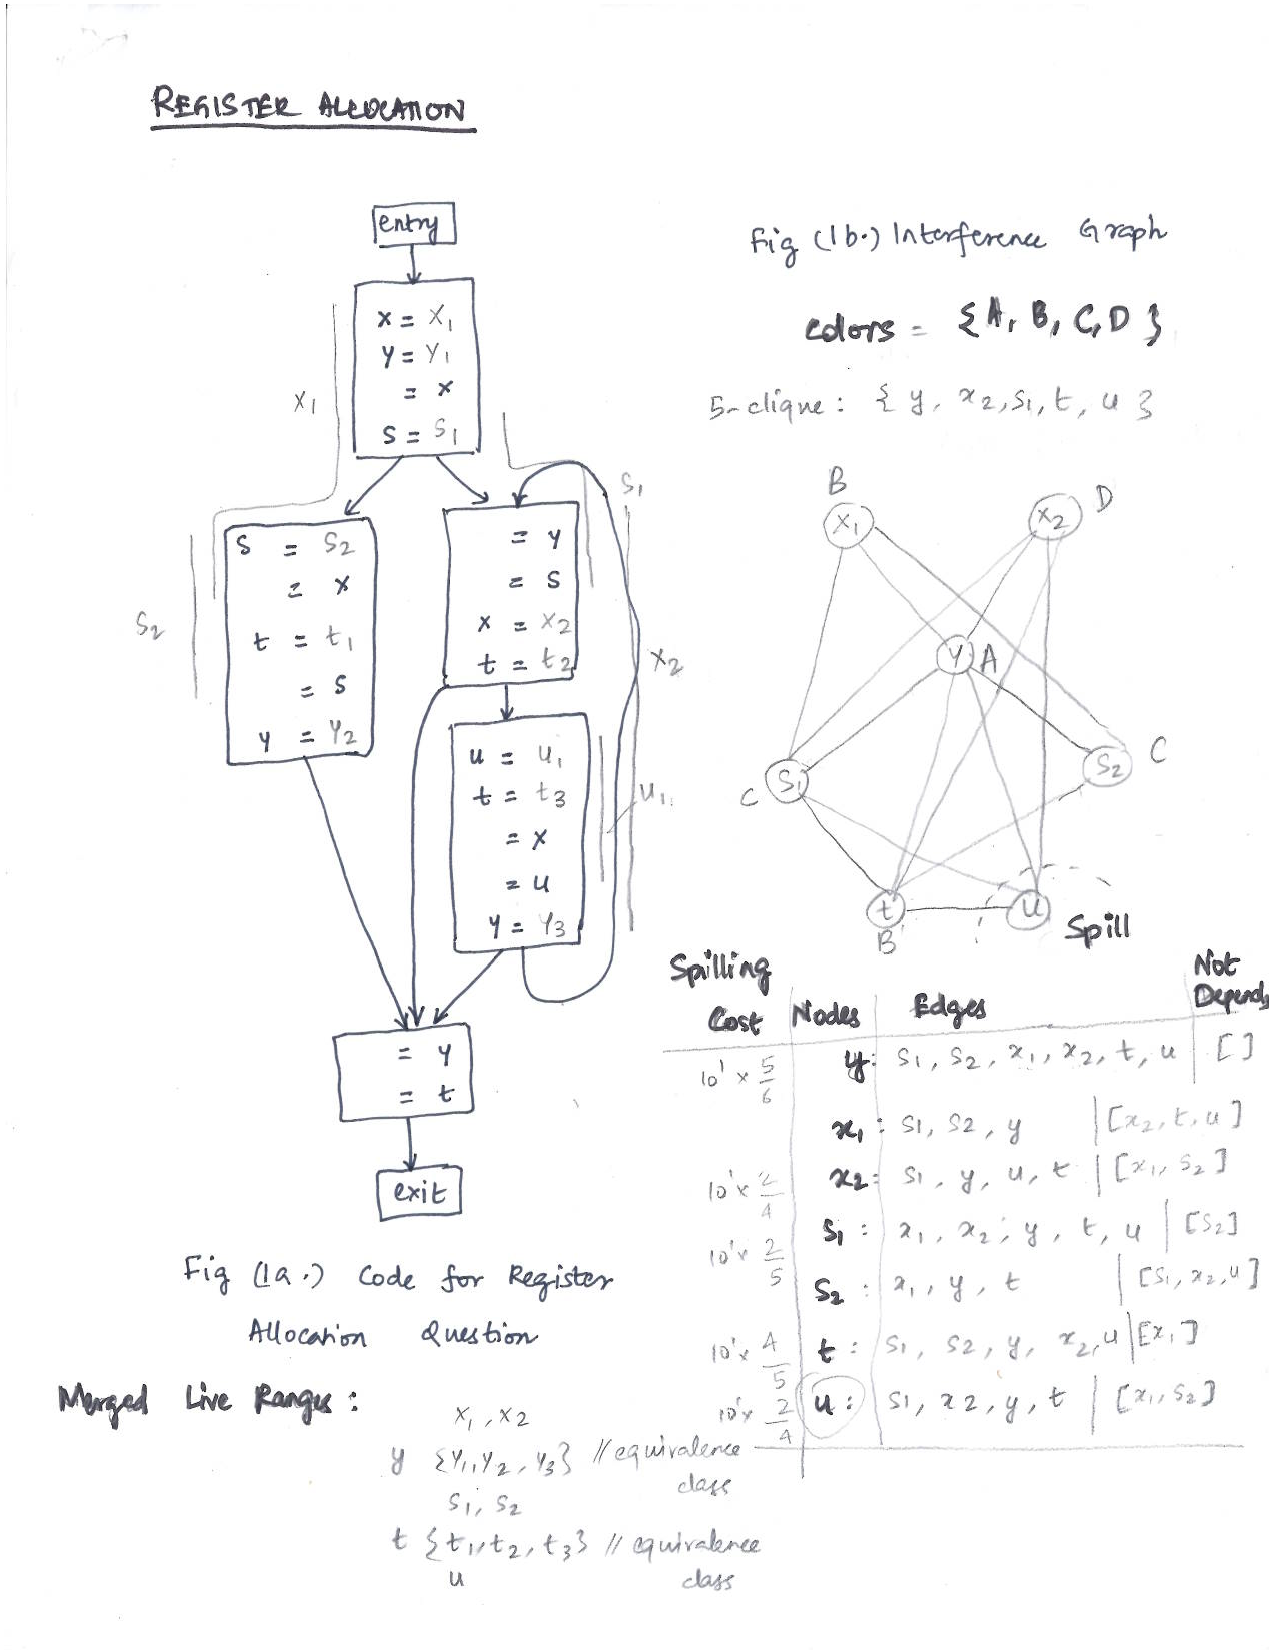
\includepdf[scale=0.7, pages={-}]{images/Q2.pdf}

%\section{LICM: Loop Invariant Code Motion}

\begin{itemize}

\item{
    \textbf{Loop-invariant instructions}\\

    The loop-invariant instructions are the following: $\{ S_{2}, S_{3}, S_{5}, S_{6}, S_{8}, S_{9}, S_{11}, S_{12} \}$.
    This is because the values of these computations  do not change as long as the control stays within the  loop.

    %These instructions are not loop-invariant : $\{ S_{1}, S_{4}, S_{7}, S_{10} \}$. They have multiple reaching definitions.
  }

  \item{
    \textbf{Loop-invariant instructions that can be moved to the pre-header}\\

    Only two instructions can be moved to the pre-header : $\{ S_{3}, S_{12} \}$. Both instructions satisfy all the three conditions required to be moved to the pre-header. In particular, $S_3$ can be moved because, while $q$ is live at the loop exit, $S_3$ dominates the loop exit. In contrast, $S_{12}$ does not dominate the loop exit, but $r$ is also not live at the loop exit. Further, when we move the two instructions to the pre-header, we must preserve their order: $S_{12}$ must be placed after $S_3$.

    The other instructions do not satisfy at least one of the three required conditions. For example, $S_5$, $S_6$, $S_9$, and $S_{11}$ cannot be moved because the variables defined by these instructions are live at the loop exit, and these instructions do not dominate the loop exit. $S_2$ and $S_8$ cannot be moved because the variables they define ($y$ and $g$ respectively) have other definitions inside the loop.
    
  }

\end{itemize}


\end{document}

%%% Local Variables:
%%% mode: latex
%%% TeX-master: "."
%%% End:
